\begin{figure}
    	\centering
    	\begin{minipage}{1\textwidth}
    			\centering
    			\begin{minipage}{0.8\textwidth}
    				\centering
    				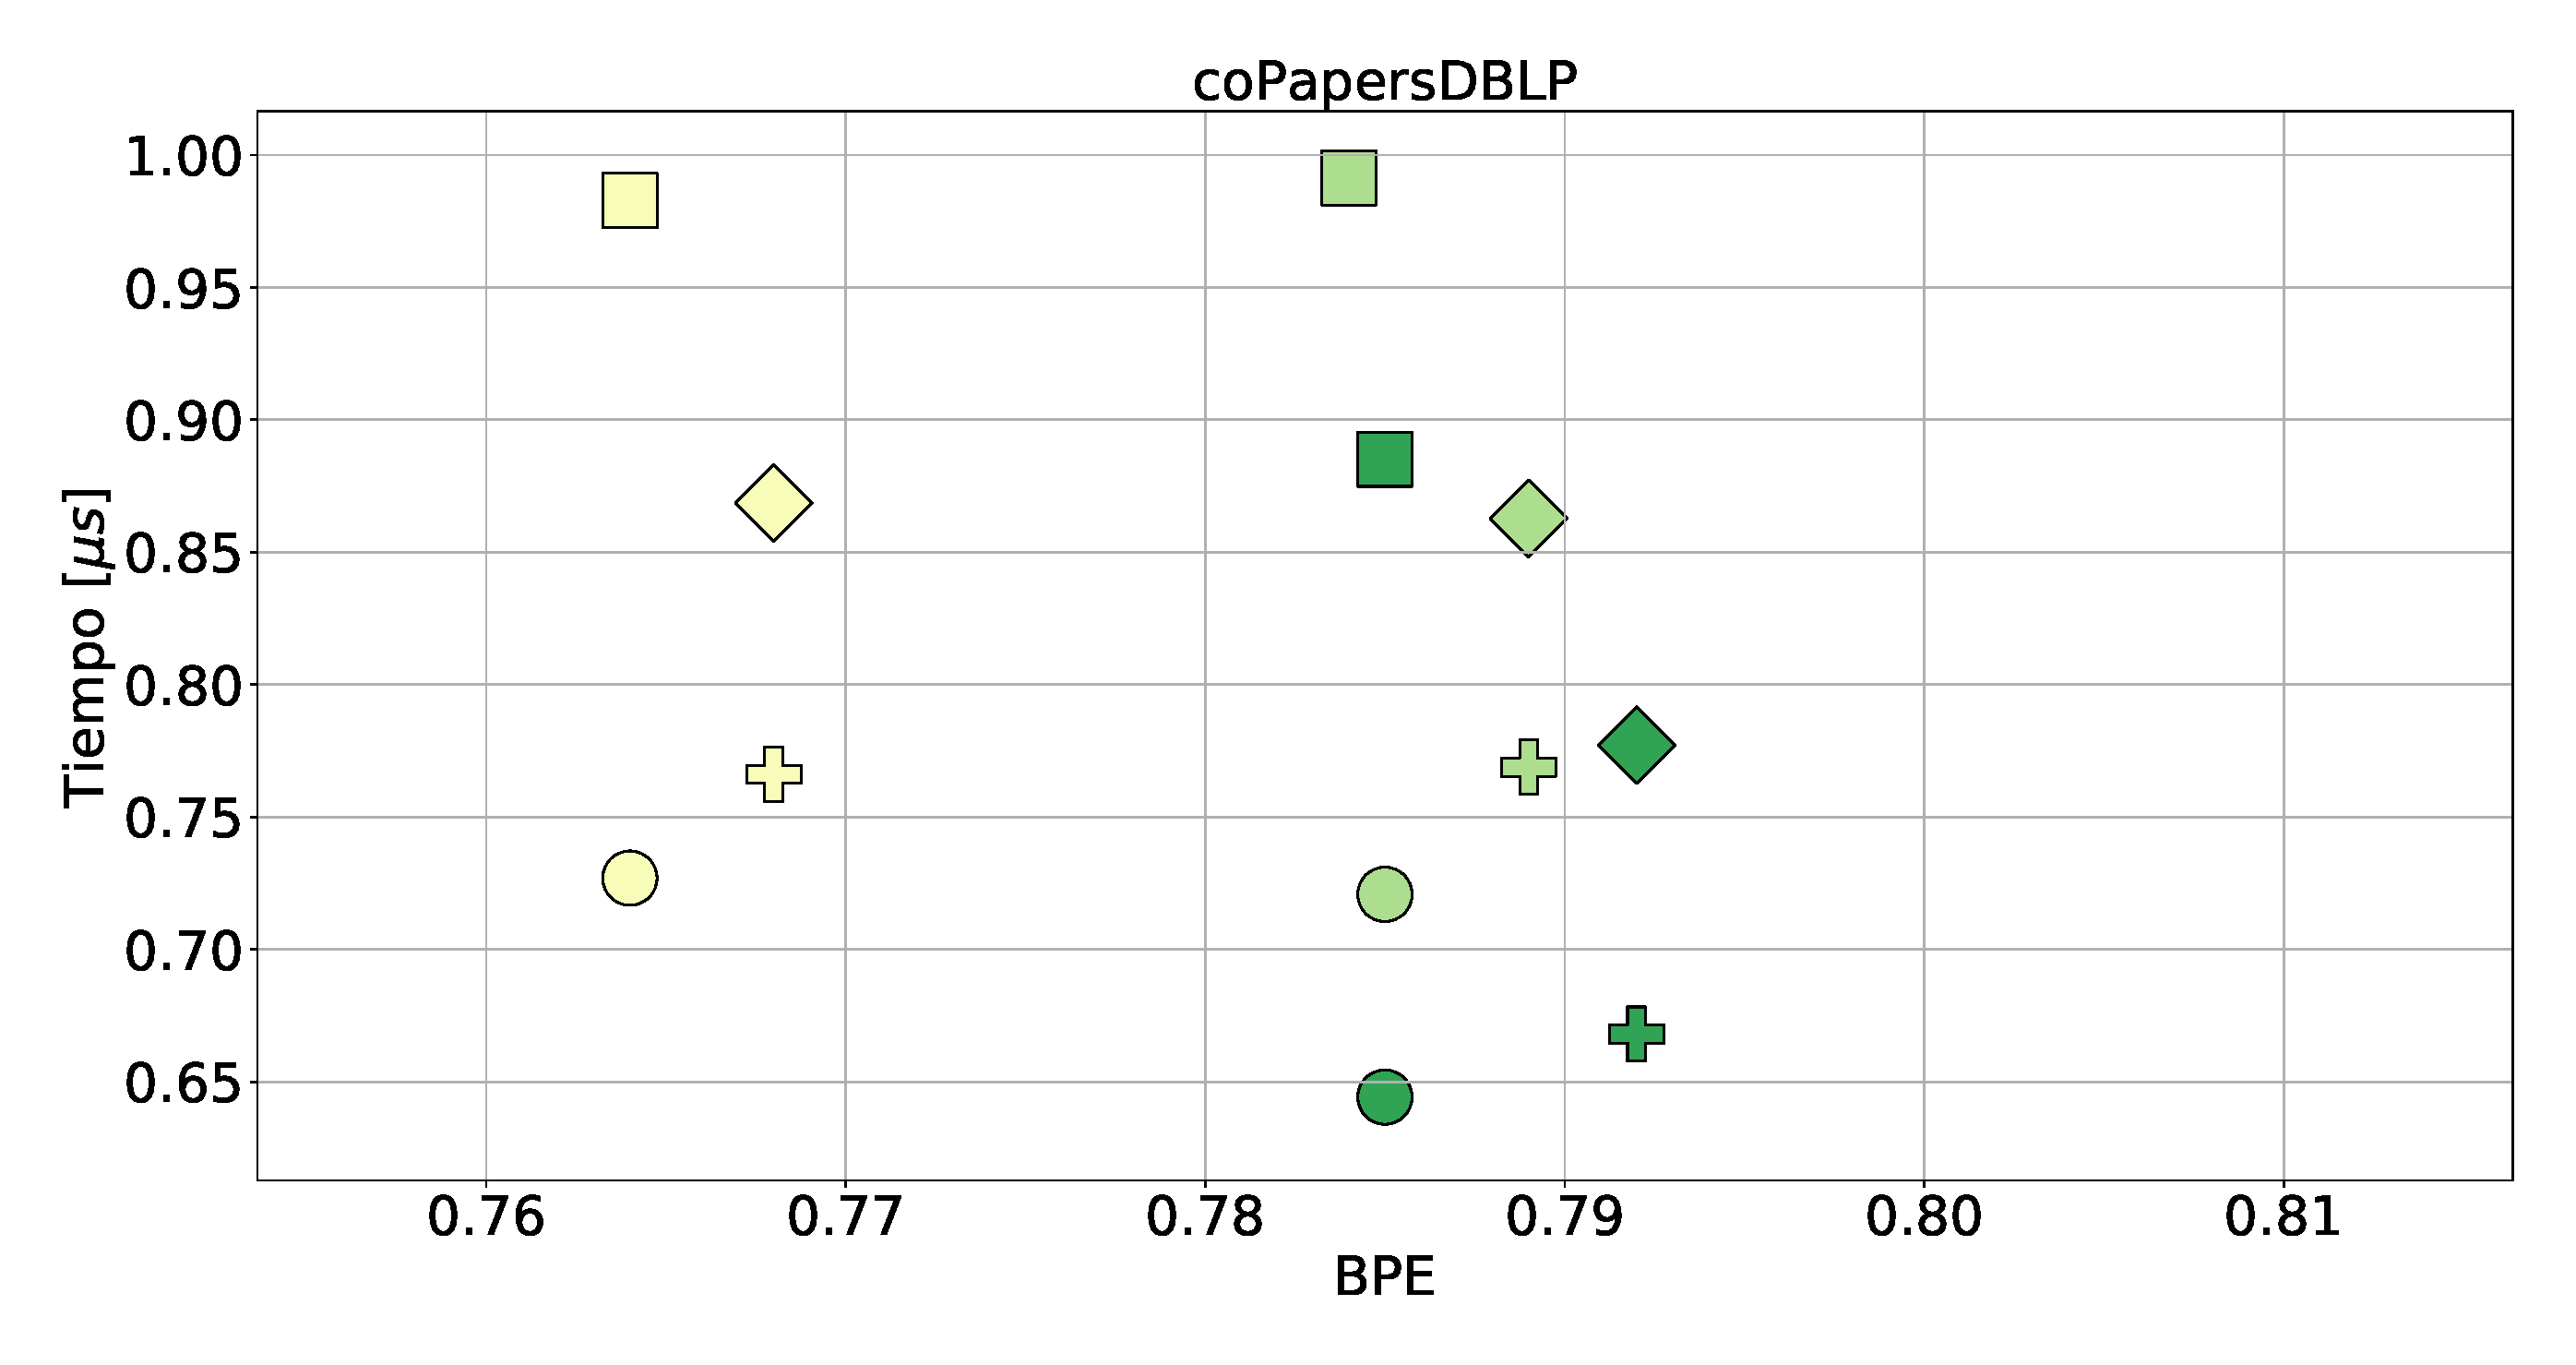
\includegraphics[width=1\linewidth]{img/sdsl/secuencialBig/coPapersDBLP.pdf}
    			\end{minipage}
    			\begin{minipage}{0.15\textwidth}
    				\centering
    				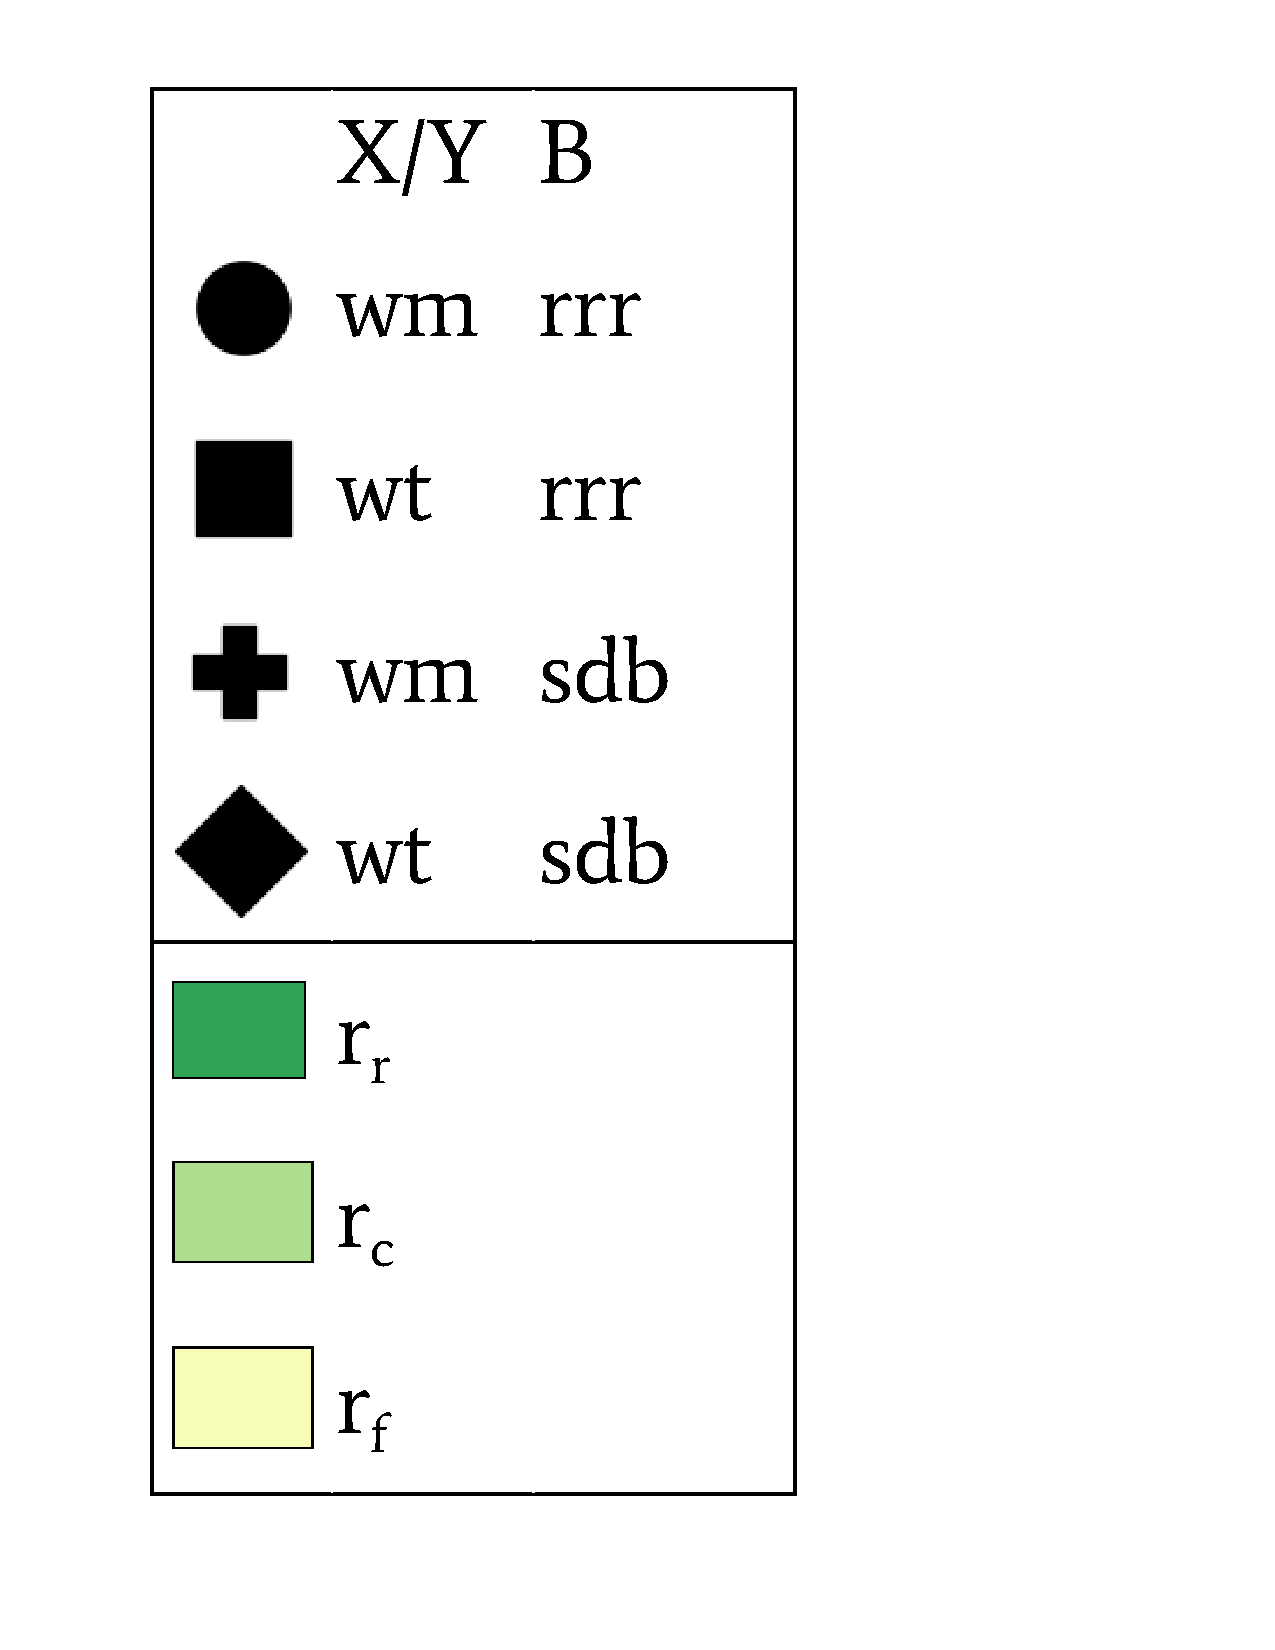
\includegraphics[scale=.22, clip, trim=70 0 0 0]{img/sdsl/label.pdf}
    			\end{minipage}
    			
    			(a)		
    	\end{minipage}
    	
       	\begin{minipage}{1\textwidth}
    			\centering
    			\begin{minipage}{0.8\textwidth}
    				\centering
    				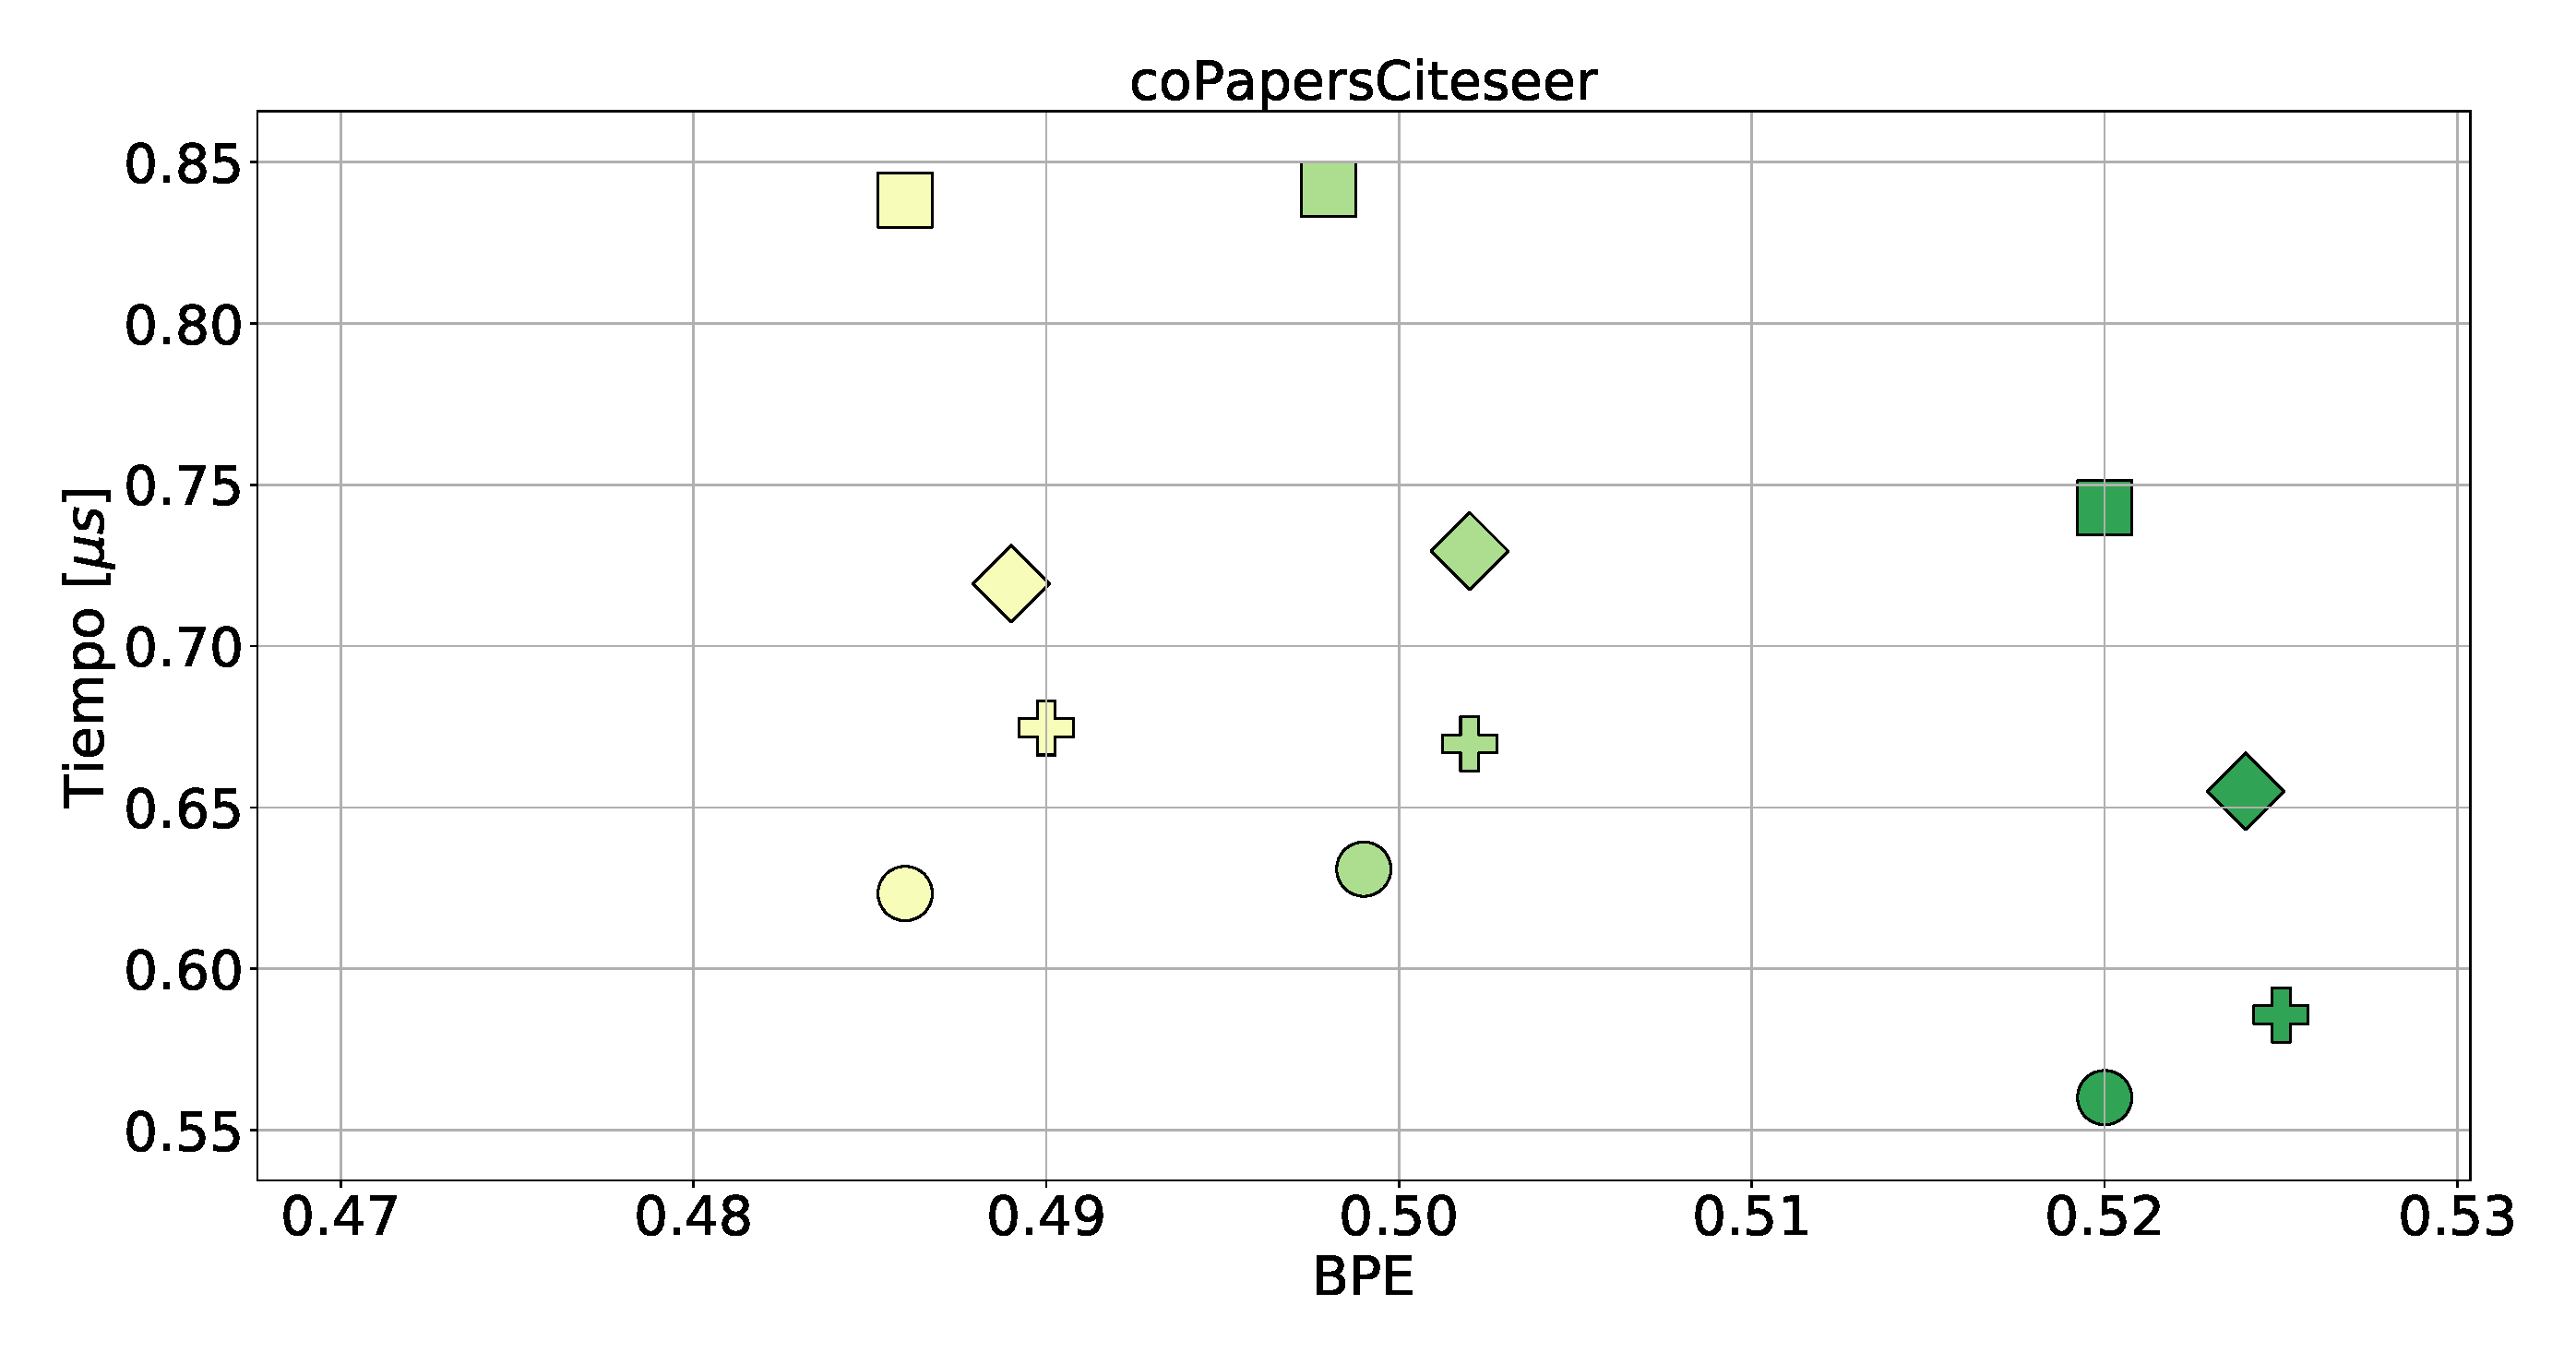
\includegraphics[width=1\linewidth]{img/sdsl/secuencialBig/coPapersCiteseer.pdf}
    			\end{minipage}
    			\begin{minipage}{0.15\textwidth}
    				\centering
    				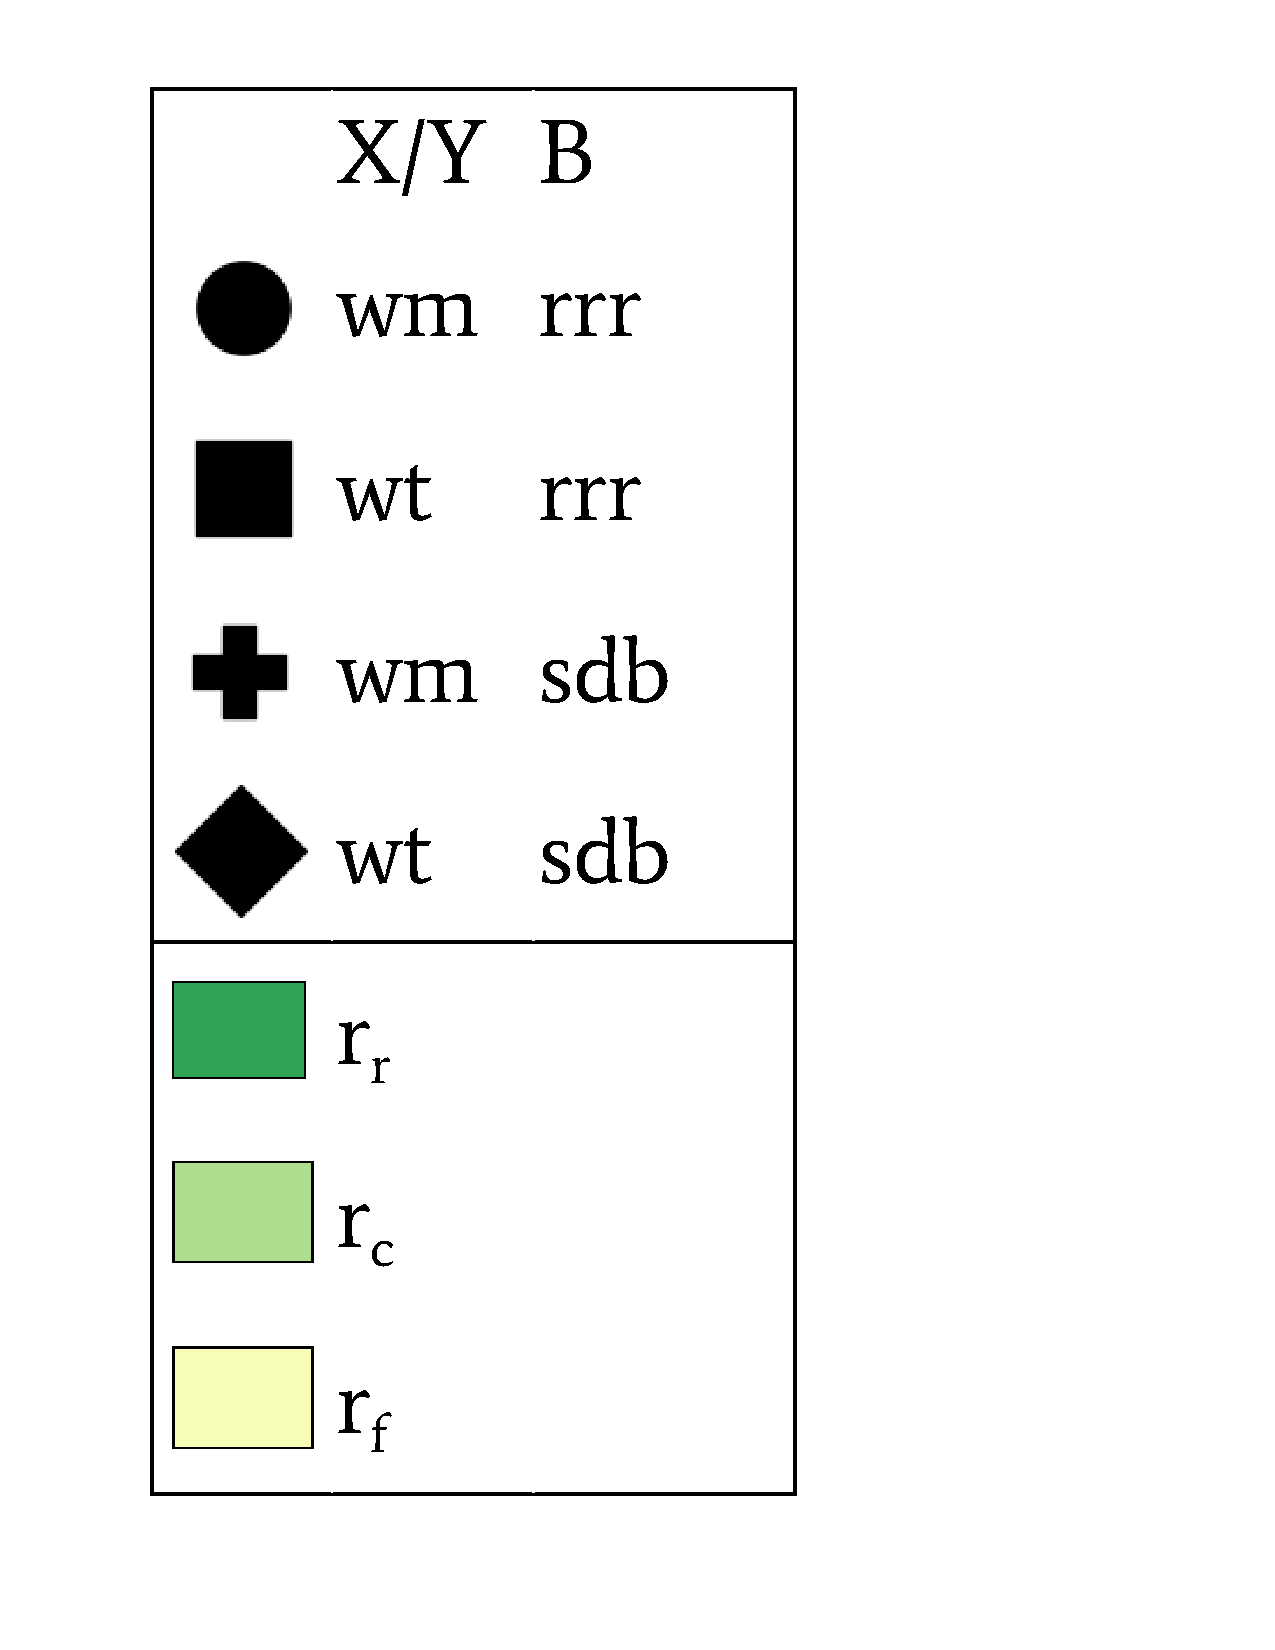
\includegraphics[scale=.22, clip, trim=70 0 0 0]{img/sdsl/label.pdf}
    			\end{minipage}
    			
    			(b)		
    	\end{minipage}
    	
    \caption{BPE y Tiempo de acceso secuencial medio para posibles estructuras compactas, por cada función de ranking, para los grafos coPapersDBLP y coPapersCiteseer.}
    \label{fig:sdslBPE5}
\end{figure}
